\chapter{Buttons and Serial Communications}
\chaplabel{buttons}

\section{Introduction}
This chapter introduces students to using buttons and serial communications.

\section{Buttons}

A typical button circuit is shown in Figure \ref{fig:buttonPullup}. The input is high until the button is pressed.
Unfortunately, being mechanical, buttons do not always create nice, clean switched inputs as is shown in 
Figure~\ref{fig:buttonDebounce}. Maxim Integrated has a 
\href{https://www.maximintegrated.com/en/design/technical-documents/app-notes/2/287.html}{nice paper} on the topic
advertizing their devices to solve the problem. However, if we don't have the option of adding their hardware, some 
work can be done in software to debounce an input. As Maxim mentions, software debouncing is not free. It does incur
some overhead so you probably do not want to do it for many inputs. Am example of software debouncing is in 
Listing \ref{lst:debounce}.

\begin{lstlisting}[language=C++, caption={This is the Arduino example of software debouncing.},label={lst:debounce}]
	/*
	Debounce
  
	Each time the input pin goes from LOW to HIGH (e.g. because of a push-button
	press), the output pin is toggled from LOW to HIGH or HIGH to LOW. There's a
	minimum delay between toggles to debounce the circuit (i.e. to ignore noise).
  
	The circuit:
	- LED attached from pin 13 to ground through 220 ohm resistor
	- pushbutton attached from pin 2 to +5V
	- 10 kilohm resistor attached from pin 2 to ground
  
	- Note: On most Arduino boards, there is already an LED on the board connected
	  to pin 13, so you don't need any extra components for this example.
  
	created 21 Nov 2006
	by David A. Mellis
	modified 30 Aug 2011
	by Limor Fried
	modified 28 Dec 2012
	by Mike Walters
	modified 30 Aug 2016
	by Arturo Guadalupi
  
	This example code is in the public domain.
  
	https://www.arduino.cc/en/Tutorial/BuiltInExamples/Debounce
  */
  
  // constants won't change. They're used here to set pin numbers:
  const int buttonPin = 9;    // the number of the pushbutton pin
  const int ledPin = 13;      // the number of the LED pin
  
  // Variables will change:
  int ledState = LOW;         // the current state of the output pin
  int buttonState;             // the current reading from the input pin
  int lastButtonState = LOW;   // the previous reading from the input pin
  
  // the following variables are unsigned longs because the time, measured in
  // milliseconds, will quickly become a bigger number than can be stored in an int.
  unsigned long lastDebounceTime = 0;  // the last time the output pin was toggled
  unsigned long debounceDelay = 50;    // the debounce time; increase if the output flickers
  
  void setup() {
	Serial.begin(115200);
	while(!Serial) delay(10);
	Serial.println("Starting...");
	
	pinMode(buttonPin, INPUT);
	pinMode(ledPin, OUTPUT);
  
	// set initial LED state
	digitalWrite(ledPin, ledState);
  }
  
  void loop() {
	// read the state of the switch into a local variable:
	int reading = digitalRead(buttonPin);
  
	// check to see if you just pressed the button
	// (i.e. the input went from LOW to HIGH), and you've waited long enough
	// since the last press to ignore any noise:
  
	// If the switch changed, due to noise or pressing:
	if (reading != lastButtonState) {
	  // reset the debouncing timer
	  lastDebounceTime = millis();
	}
  
	if ((millis() - lastDebounceTime) > debounceDelay) {
	  // whatever the reading is at, it's been there for longer than the debounce
	  // delay, so take it as the actual current state:
  
	  // if the button state has changed:
	  if (reading != buttonState) {
		buttonState = reading;
  
		// only toggle the LED if the new button state is HIGH
		if (buttonState == HIGH) {
		  ledState = !ledState;
		}
	  }
	}
  
	// set the LED:
	digitalWrite(ledPin, ledState);
  
	// save the reading. Next time through the loop, it'll be the lastButtonState:
	lastButtonState = reading;
  
  }
\end{lstlisting}

\begin{figure}[!htb]
	\centering
	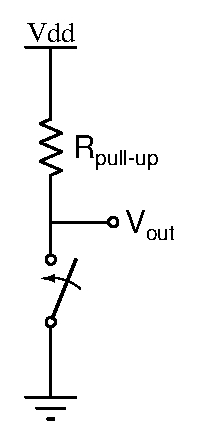
\includegraphics{buttonSerial/button1.eps}
	\caption{This is a typical button input circuit. It is active low in that the output signal will be high until the button is pressed.}
	\label{fig:buttonPullup}
\end{figure}

\begin{figure}[!htb]
	\centering
	\includegraphics[scale=0.5]{buttonSerial/debounce.eps}
	\caption{This is an example of what the output signal from a button with the circuit in Figure \ref{fig:buttonPullup} could look like.}
	\label{fig:buttonDebounce}
\end{figure}


\section{Serial Communications}
Serial communications sends data one bit at a time from one device to another as shown in Figure \ref{fig:serial}. This is in 
contrast to parallel communications where multiple bits (8 in the example) are transferred simultaneously between devices as 
shown in Figure \ref{fig:parallel}. As can be seen parallel communications is much faster than serial since you can send 
so many bits simultaneously. However, parallel requires many more pins on each device to communicate. This is challenging in 
the embedded systems world since most microcontrollers don't have many pins. Also, connectors with many pins tend to fail 
more often than connectors with fewer pins. Because of these reasons, the embedded world communicates primarily with serial 
protocols. 

\begin{figure}[!htb]
	% Serial
	\centering
	\begin{tikzpicture}
		% BLOCKS
		\draw[thick] (0,0) rectangle (4,4) node (dev1) [pos=0.5] {Device 1};
		\draw[thick] (8,0) rectangle (12,4) node (dev2) [pos=0.5] {Device 2};
		% ARROWS	
		\draw [thick,-{latex[length=4mm, width=6mm]}] (4,2) |- node [above,pos=0.75] {01101101} (8,2) ;
	\end{tikzpicture}
	\caption{Serial transfers one bit at a time.}
	\label{fig:serial}
\end{figure}
	
	% Parallel
\begin{figure}[!htb]
	\centering
	\begin{tikzpicture}
		% BLOCKS
		\draw[thick] (0,0) rectangle (4,5) node (dev3) [pos=0.5] {Device 1};
		\draw[thick] (8,0) rectangle (12,5) node (dev4) [pos=0.5] {Device 2};
		% ARROWS	
		\draw [thick,-{latex[length=4mm, width=6mm]}] (4,4.25) |- node [above,pos=0.75] {0} (8,4.25) ;
		\draw [thick, -{latex[length=4mm, width=6mm]}] (4,3.75) |- node [above,pos=0.75] {1} (8,3.75) ;
		\draw [thick, -{latex[length=4mm, width=6mm]}] (4,3.25) |- node [above,pos=0.75] {1} (8,3.25) ;
		\draw [thick, -{latex[length=4mm, width=6mm]}] (4,2.75) |- node [above,pos=0.75] {0} (8,2.75) ;
		\draw [thick, -{latex[length=4mm, width=6mm]}] (4,2.25) |- node [above,pos=0.75] {1} (8,2.25) ;
		\draw [thick, -{latex[length=4mm, width=6mm]}] (4,1.75) |- node [above,pos=0.75] {1} (8,1.75) ;
		\draw [thick, -{latex[length=4mm, width=6mm]}] (4,1.25) |- node [above,pos=0.75] {0} (8,1.25) ;
		\draw [thick, -{latex[length=4mm, width=6mm]}] (4,0.75) |- node [above,pos=0.75] {1} (8,0.75) ;
		
	\end{tikzpicture}
	\caption{Parallel transfers multiple bits at a time.}
	\label{fig:parallel}
\end{figure}

A table of serial protocols is listed in Table \ref{table:serialTypes}. 

\begin{table}[!ht]
	\centering
	\begin{tabular}{l l}
		\hline
		Protocol & Description \\ 
		\hline
		UART & Used to communicate between computers and Arduino boards \\
		SPI & Used for higher speed communications between devices on circuit boards \\
		I\textsuperscript{2}C & Only uses two wires and allows for multiple controllers and peripherals \\
		\rowcolor{lightgray}\emph{CAN} & \emph{Often used in the automotive industry} \\
		\rowcolor{lightgray}\emph{RS-485} & \emph{Differential signaling for robustness (noisy and long wires)} \\
		\rowcolor{lightgray}\emph{1-Wire}  & \emph{Only requires 1 wire and ground (no power) to communicate} \\
		\rowcolor{lightgray}\emph{USB} & \emph{Ubiquitous on computers now} \\
		\hline
	\end{tabular}
	\caption{This is a list of some of the more common serial protocols. The grayed out protocols will not be discussed further.}
	\label{table:serialTypes}
\end{table}

\subsection{Universal Asynchronous Receiver-Transmitter}
The Universal Asynchronous Receiver-Transmitter (UART) protocol has been around quite a while. Older computers used to ship with
serial ports that used this protocol, usually implemented as the RS-232 protocol. UARTs are used to communicate between two devices.
It does not allow for more than two devices. It is full duplex and communicates over 2 wires (plus a ground for reference). 
One wire transmits data from Device 1 to Device 2 and is connected to Device 1's TX pin and Device 2's RX pin. The second wire 
transmits data from Device 2 to Device 1 and is connected to Device 1's RX pin and Device 2's TX pin. This is illustrated in 
Figure \ref{fig:uart}. This protocol does require both devices to use the same specified transmission speed. Some common speeds
are 9600, 14,400, 57,600, and 115,200. It can go faster. Nowadays, it is generally best to go as fast as possible so that
the communications takes less of the processor's time. The most common speed used now seems to be 115,200. The asynchronous 
part of the name comes from the fact that there is no clock line for UARTs. It typically has a maximum speed of 1.5 megabits 
per second (Mbps).

UART is the protocol used to communicate between the computer and your Arduino board. You can see this in the code 
in the setup function where \lstinline{Serial.begin(115200)} or \lstinline{Serial.begin(9600)} shows up often.

\begin{figure}[!htb]
	% UART
	\centering
	\begin{tikzpicture}
		% BLOCKS
		\draw[thick] (0,0) rectangle (4,4) node (dev1) [pos=0.5] {Device 1};
		\draw[thick] (8,0) rectangle (12,4) node (dev2) [pos=0.5] {Device 2};
		% ARROWS	
		\draw [thick,-{latex[length=4mm, width=6mm]}] (4,2.5) node [anchor=east] {TX} -- (8,1.5) node [anchor=west] {RX} ;
		\draw [thick,{latex[length=4mm, width=6mm]}-] (4,1.5) node [anchor=east] {RX} -- (8,2.5) node [anchor=west] {TX} ;
	\end{tikzpicture}
	\caption{A UART has full duplex between two entities.}
	\label{fig:uart}
\end{figure}

\subsection{Serial Peripheral Interface}
The Serial Peripheral Interface (SPI) is a full-duplex serial interface shown in Figure \ref{fig:spi}. It is setup in a controller-peripheral 
(previously known as master-slave) architecture with only one controller on the bus. It does allow for multiple 
peripherals by giving each peripheral its own chip select (CS) line. Since it is synchronous, it does require a
clock line. This means that it takes a minimum of 4 wires as listed in Table \ref{table:spiwires}. The SCLK signal is the
clock signal used by both the controller and peripheral. There is one CS line per peripheral. The CS line lets the controller 
specify which peripheral it is communicating with. The COPI line is the data going from the controller to the peripheral. 
The CIPO line is the data going from the peripheral to the controller. 

SPI has a maximum data rate of 60 Mbps, which is the fastest of the 3 protocols commonly used in the embedded world. Because of 
this, it is used in more data intense situations like SD Cards (where we will be using it) and displays.

\begin{figure}[!htb]
	% SPI
	\centering
	\begin{tikzpicture}
		% BLOCKS
		\draw[thick] (0,-1.5) rectangle (4,3.5) node (dev1) [anchor=east,pos=0.6] {Controller};
		\draw[thick] (9,-1) rectangle (12,4) node (dev2) [pos=0.5] {Peripheral 1};
		\draw[thick] (9, -2) rectangle (12,-6) node (dev3) [pos=0.5] {Peripheral 2};
		% ARROWS	
		\draw [thick,-{latex[length=4mm, width=6mm]}] (4,3) node [anchor=east] {CS1} |- (9,3) node [anchor=west] {CS} ;
		\draw [thick,-{latex[length=4mm, width=6mm]}] (4,2) node [anchor=east] {SCLK} -- (9,2) node [anchor=west] {SCLK} ;
		\draw [thick,-{latex[length=4mm, width=6mm]}] (4,1) node [anchor=east] {COPI} -- (9,1) node [anchor=west] {COPI} ;
		\draw [thick,{latex[length=4mm, width=6mm]}-] (4,0) node [anchor=east] {CIPO} -- (9,0) node [anchor=west] {CIPO} ;
		\draw [thick,-{latex[length=4mm, width=6mm]}] (4,-1) node [anchor=east] {CS2} |- (5,-1) |- (9,-5.5) node [anchor=west] {CS} ;
		\draw [thick, -{latex[length=4mm, width=6mm]}] (8,2) |- (9,-2.5) node [anchor=west] {SCLK} ;
		\draw [thick, -{latex[length=4mm, width=6mm]}] (7,1) |- (9,-3.5) node [anchor=west] {COPI} ;
		\draw [thick] (6,0) |- (9,-4.5) node [anchor=west] {CIPO} ;
		\fill[black]  (8,2) circle (3pt) ;  % SCLK
		\fill[black]  (7,1) circle (3pt) ;  % COPI
		\fill[black]  (6,0) circle (3pt) ;  % CIPO
	\end{tikzpicture}
	\caption{SPI allows for one (sometime more) controller and multiple peripherals.}
	\label{fig:spi}
\end{figure}

\begin{table}[!ht]
	\centering
	\begin{tabular}{l l}
		\hline
		Signal & Description \\ 
		\hline
		SCLK & Clock signal to keep everything synchronized \\
		CS & Chip select--tells a peripheral that the controller is communicating with it \\
		COPI & Controller Out, Peripheral In (used to be MOSI) \\
		CIPO & Controller In, Peripheral Out (used to be MISO) \\
		\hline
	\end{tabular}
	\caption{The SPI protocol uses these signals to connect.}
	\label{table:spiwires}
\end{table}

\subsection{Inter-Integrated Circuit}
The Inter-Integrated Circuit (I\textsuperscript{2}C, IIC, or I2C) protocol is multi-controller and multi-peripheral. Basically,
any device connected to the bus can drive the communication. It is single ended so data only flows one way at a time. It only 
requires 3 wires, SCL - clock, SDA - Data, and a ground reference. SCL and SDA do require pull-up resistors so that devices
only have to pull the lines to ground to communicate as shown in Figure \ref{fig:i2c}. Instead of using chip select lines 
like SPI, I2C requires each peripheral to have a unique address. I2C addresses for modules that are on the board or may be 
used with the board can be seen in Table \ref{table:i2caddresses}. I2C has a max speed of 3.4 Mbps but is only 100 kbps in 
standard mode.

\begin{figure}[!htb]
	% I2C
	\centering
	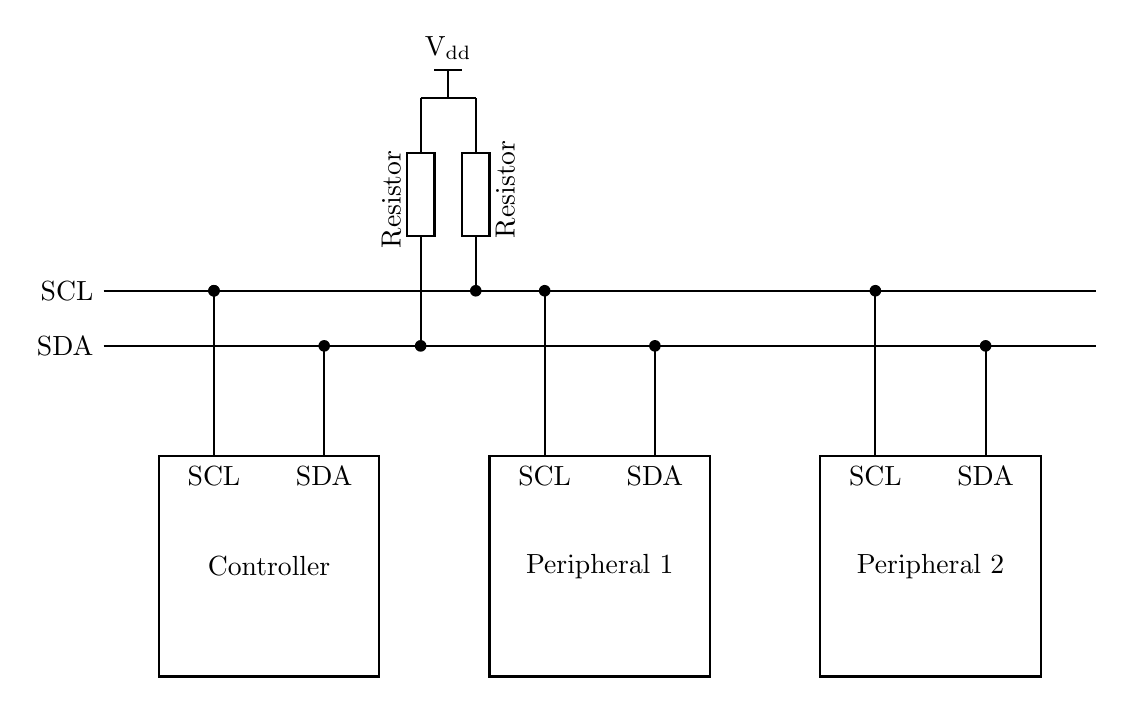
\begin{tikzpicture}[scale=0.7]
		% BLOCKS
		\draw[thick] (0,0) rectangle (4,4) node (dev1) [pos=0.5] {Controller};
		\draw[thick] (6,0) rectangle (10,4) node (dev2) [pos=0.5] {Peripheral 1};
		\draw[thick] (12, 0) rectangle (16,4) node (dev3) [pos=0.5] {Peripheral 2};
		\draw[thick] (4.5, 8) rectangle (5,9.5) node (r1) [above=2ex,pos=0.15, rotate=90] {Resistor};
		\draw[thick] (5.5, 8) rectangle (6,9.5) node (r2) [below=2ex,pos=0.85, rotate=90] {Resistor};
		
		% ARROWS	
		\draw [thick] (-1,6) node [anchor=east] {SDA} -- (17,6) ;
		\draw [thick] (-1,7) node [anchor=east] {SCL} -- (17,7)  ;
		\draw [thick] (1,4) node [anchor=north] {SCL} -- (1,7) ;
		\draw [thick] (3,4) node [anchor=north] {SDA} -- (3,6) ;
		\draw [thick] (7,4) node [anchor=north] {SCL} -- (7,7) ;
		\draw [thick] (9,4) node [anchor=north] {SDA} -- (9,6) ;
		\draw [thick] (13,4) node [anchor=north] {SCL} -- (13,7) ;
		\draw [thick] (15,4) node [anchor=north] {SDA} -- (15,6) ;
		\fill[black]  (1,7) circle (3pt) ;
		\fill[black]  (1,7) circle (3pt) ;
		\fill[black]  (7,7) circle (3pt) ;
		\fill[black]  (13,7) circle (3pt) ;
		\fill[black]  (3,6) circle (3pt) ;
		\fill[black]  (9,6) circle (3pt) ;
		\fill[black]  (15,6) circle (3pt) ;
		\draw [thick] (4.75,6)  -- (4.75,8) ;
		\fill[black]  (4.75,6) circle (3pt) ;
		\draw [thick] (5.75,7)  -- (5.75,8) ;
		\fill[black]  (5.75,7) circle (3pt) ;
		\draw [thick] (5.75,9.5)  -- (5.75,10.5) ;
		\draw [thick] (4.75,9.5)  -- (4.75,10.5) ;
		\draw [thick] (4.75,10.5)  -- (5.75,10.5) ;
		\draw [thick] (5.25,10.5)  -- (5.25,11) ;
		\draw [thick] (5,11)  -- node [above,pos=0.5] {V\textsubscript{dd}} (5.5,11) ;
	\end{tikzpicture}
	\caption{I\textsuperscript{2}C allows for multiple controllers and peripherals on the same bus.}
	\label{fig:i2c}
\end{figure}


\begin{table}[!ht]
	\centering
	\begin{tabular}{l l}
		\hline
		Address (HEX) & Module \\ 
		\hline
		0x44 or 0x45 & SHT31-DIS Temperature/Humidity \\
		0x3D & 1.3" 128x64 OLED Display \\
		0x39 & APDS-9960 Light, Color, Proximity, Gesture \\
		0x77 & BME688 Temperature, Humidity, Gas \\
		0x2D, 0x53, and 0x57 & ST25DV16 Dynamic NFC/RFID Tag IC \\
		0x30 or other  & NeoKey 1x4 QT breakout board \\
		0x10 & STEMMA MiniGPS \\
		0x6A or 0x6B & LSM6DSOX IMU on the Nano Connect \\
		0x60  & ATECC608A Cryptographic on the Nano Connect \\
		\hline
	\end{tabular}
	\caption{I2C addresses for relevant modules.}
	\label{table:i2caddresses}
\end{table}

\section{In Case of Upload Lock-up or Failure}
If the Arduino IDE is having trouble uploading to the Arduino Nano RP2040 Connect, try double pressing
(not too fast) the reset button on the Nano once the IDE starts trying to upload.

\section{Arduino Programming Suggestions}
In general, try to start from an existing set of code (an example for instance) when working on something.
For example, if you need to use the APDS-9960, load one of the examples from the library, then modify it
until it does what you want. Once you have written a few sketches, you might write a generic starting point
for your subsequent sketches.

\section{Arduino Button Setup}
An example of how to setup the buttons on the CEC 325 board. Some important details to note is that the left button 
is attached to pin D9 (referred to as 9 in the Arduino infrastructure) which is attached to the RP2040 on the
Arduino Nano RP2040 Connect module. The RP2040 has internal pull-up resistors that are tied correctly to the 
Arduino IDE so that the pins can be setup using \lstinline@pinMode(LEFT_BUTTON_PIN, INPUT_PULLUP);@ and do not
require an external pull-up resistor. The right button is attached to pin A7 on the module which is routed to the
WiFiNINA module. This module's internal pull-up is not implemented in the Arduino IDE (as of 2022 February 03). 
Therefore, it needs an external pull-up AND requires the sketch to include "WiFiNINA.h" AND the pin variable 
HAS to be declared using \lstinline@#define@ rather than a \lstinline@const int@.

\begin{lstlisting}[language=C++, caption={This is an example of how to setup the buttons on the CEC 325 board.},label={lst:buttons}]
/* button_demo.ino
 *  
 *  Gives an example of how to use the buttons on 
 *  the CEC 325 board.
 *  
 *  Seth McNeill
 *  2022 February 03
 */

#include "WiFiNINA.h"  // for A4-A7 and wifi/bluetooth

#define LEFT_BUTTON_PIN   9 // This input is on the RP2040 and has builtin pullup that works
#define RIGHT_BUTTON_PIN  A7 // This input is on the WiFiNINA and doesn't have working internal pullup

void setup() {
  Serial.begin(115200);
  //while(!Serial) delay(10);
  delay(2000);

  Serial.println("Starting...");

  pinMode(LEFT_BUTTON_PIN, INPUT_PULLUP);
  pinMode(RIGHT_BUTTON_PIN, INPUT);
  pinMode(LED_BUILTIN, OUTPUT);
}

void loop() {
  // note that the buttons read 1 (HIGH or true) when not pressed
  if(!digitalRead(LEFT_BUTTON_PIN)) {
    Serial.println("Left button pushed");
  }
  if(!digitalRead(RIGHT_BUTTON_PIN)) {
    Serial.println("Right button pushed");
  }
  delay(100); // keeps the loop from running too fast with nothing pushed
}
\end{lstlisting}

\section{Arduino Serial Setup}
The serial port has to be setup in the \lstinline@setup()@ function in the Arduino IDE. An example of setting it up 
is shown in Listing \ref{lst:serial}.

\begin{lstlisting}[language=C++, caption={This is an example of how to start the serial port at 112,500 in the Arduino system.},label={lst:serial}]
void setup() {
  Serial.begin(115200); // starts the serial connection at 115200 data (baud) rate
  // If you are attached to a computer (not a robot on battery power
  while(!Serial) delay(10); // wait for serial to start
  // delay(2000);  // if might be on battery, just wait a bit for it to start
  Serial.println("Starting...");

}

void loop() {
  Serial.println("This has a new line character at the end");
  Serial.print("This does not have a new line at the end: ");
  Serial.println(millis());
  delay(5000);
}
\end{lstlisting}
I strongly suggest having the \lstinline@setup()@ function output to the serial port right after the serial port is started 
so that you can know that your board has booted. Note that if you do not have a serial port (your robot is running off of 
batteries so that it is not plugged into a computer) you need to remove the \lstinline@while(!Serial) delay(10)@ line and 
replace it with some sort of timeout function. A \lstinline@delay(2000)@ is usually sufficient to allow the serial to start 
if it exists but not hang if it doesn't. There are more complicated ways to do this, but that will be left as an exercise 
for the reader.


\section{Laboratory Exercises}
\subsection{Button to Serial}
Create a sketch that prints to the serial port at 115,200 each time a button is pressed. The message should indicate which
button is pressed. Both buttons should work on your board. Don't forget that the right button (A7) requires WiFiNINA.h to
be included and the pin designation to be a \lstinline@#define@ not a \lstinline@const int@. The error messages are pretty helpful on this.

\subsection{Tones}
Create a sketch that plays a short tune when one of the buttons is pressed. There are examples of using the \lstinline@tone@ 
function in Examples $\rightarrow$ 02.Digital. The buzzer is attached to pin A2 on the Arduino Nano RP2040 Connect.

\subsection{APDS-9960}
Create a sketch that prints the distance and color to the serial port once a second. In order to get the APDS-9960 working,
you will need to install a library for it. Arduino, Adafruit, and Sparkfun all have libraries available in the library 
manager. I have been using the Arduino one. Once you install the library, a new folder on the Examples menu should show up. 
Look through the examples to get an idea how to do this. 

\subsection{Distance to Tone}
Create a sketch that plays an increasing tone as the APDS-9960's distance measurement decreases. It should play 
no tone if there is nothing nearby (sensor reading 255 from the Arduino library). 

\subsection{Color Recognition}
Create a sketch that plays a tone or turns on a light (LED) when a specific color is seen by the APDS-9960. My playing with 
the color readings is that it is not very precise. It is probably best to choose colors and just react to redder colors or 
something down that line.

\subsection{SHT31}
Install the Adafruit SHT31 library and run it to see the temperature and humidity.

%\subsection{Detecting Human Breathing}
%Create a sketch that turns on a light or plays a tone when someone breathes on the SHT31 sensor.

\subsection{Turn In}
After demonstrating each sketch to the instructor, submit a copy of all the sketches compiled into a single PDF to Canvas. Also, submit the sketch files. Be sure that each sketch has the following 
header:
\begin{lstlisting}
/* sketch_name.ino
 *
 * A description of what the sketch does 
 *   and the inputs/outputs it needs.
 *
 * All authors' names (if working with a 
 *   partner be sure to include both your names)
 * CEC 326 (or other class name)
 * Today's date in the format YYYY mmmmm dd 
 *   as in 2022 February 03
 */
\end{lstlisting}